\documentclass[hyperref=colorlinks]{beamer}
\mode<presentation>
\usetheme{iclpt}
\setbeamertemplate{navigation symbols}{}
\setbeamertemplate{headline}{
\begin{beamercolorbox}[leftskip=.2cm,rightskip=.2cm,topskip=.2cm,ht=1.1cm,dp=0.1cm,wd=\textwidth]{institute in head/foot}
  
\includegraphics[height=1cm]{icl.pdf}
  \hfill
  
\includegraphics[height=1cm]{../Pics/CMS-Color.pdf}
\end{beamercolorbox}
}
\setbeamertemplate{footline}{
\begin{beamercolorbox}[ht=.55cm,dp=0.4cm,wd=\textwidth,leftskip=.3cm]{author in head/foot}%
  \begin{minipage}[c]{5cm}%
    \usebeamerfont{author in head/foot}
    \insertshortauthor 
    \insertshorttitle
    \end{minipage}\hfill%
  \insertframenumber{} / \pageref{lastframe}
  \hfill
  \begin{minipage}{6cm}
    \hfill
  \end{minipage}
\end{beamercolorbox}%
}

\usepackage{color}
\usepackage{tabularx,colortbl}
\usepackage{graphicx}
\usepackage{pdfpages}
\usepackage{feynmp}
\DeclareGraphicsRule{*}{mps}{*}{}

\title{\vspace{-0.2cm} VBF Higgs to Invisible}
\subtitle{HIG-14-038, AN-14-243\vspace{-0.7cm}}
\author[P. Dunne]{\underline{P. Dunne}} % A.M. Magnan and A. Nikitenko Joao Pela with \\ R. Aggleton, J. Brooke: Bristol \\ C.Asawangtrakuldee, Q.Li: Peking \\ P. Srimanobhas: Chulalongkorn \\ S. Kumar, K. Mazumdar: Mumbai}
\titlegraphic{
  \vspace{-0.7cm}
  %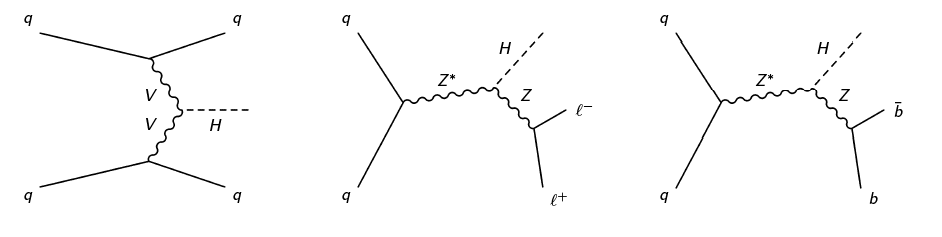
\includegraphics[width=\textwidth]{TalkPics/invcomb021213/feyndiags}
  %% \begin{fmfgraph*}(100,70)
  %%         \fmfleft{i1,i2}
  %%         \fmfright{o1,o2,o3}
  %%         \fmf{fermion}{i1,v1,o1}
  %%         \fmf{fermion}{i2,v2,o3}
  %%         \fmf{phantom,tension=4/5}{v1,v2}
  %%         \fmffreeze
  %%         \fmf{photon,label=$W,,Z$}{v1,v3}
  %%         \fmf{photon,label=$W,,Z$}{v2,v3}
  %%         \fmf{dashes}{v3,o2}
  %%         \fmflabel{$q$}{i1}
  %%         \fmflabel{$q$}{i2}
  %%         \fmflabel{$q$}{o1}
  %%         \fmflabel{$q$}{o3}
  %%         \fmflabel{$H$}{o2}
  %%       \end{fmfgraph*}
}
\date{}
\begin{document}
\begin{fmffile}{higgsexoupdatefeyndiags}

%TITLE PAGE
\section{Title}
\begin{frame}
  \titlepage
  
\end{frame}

\begin{frame}
  \frametitle{Overview}
  \begin{block}{}
    \scriptsize
    \begin{itemize}
    \item Pub comm and physics coordination intend that our result is made public as a PAS only
    \item There are a few points we would like to make them aware of before this decision is finalised:
    \item[-] We hope to reduce the uncertainty on the $Z\rightarrow\nu\nu$ background from the extrapolation from the $Z\rightarrow\mu\mu$ region
    \item[-] The final limit from combining with the ZH channel searches is also significantly improved
    \item[-] This is not an intermediate result, due to reduced trigger acceptance we don't expect to improve our expected limit until at least the end of 2016
    \end{itemize}
  \end{block}
\end{frame}

\begin{frame}
  \frametitle{VBF only limit}
  \vspace{-.35cm}
  \begin{columns}
    \column{1.1\textwidth}
    \begin{block}{}
      \scriptsize
    \begin{itemize}
    \item We hope to improve the $Z/\gamma^{*}\rightarrow\mu\mu$ to $Z\rightarrow\nu\nu$ extrapolation uncertainty
    \item[-] This could double our improvement in expected limit over the prompt analysis
    \item[-] It could allow us to reproduce the prompt data combined limit in the VBF channel alone
    \end{itemize}
        
    \centering
    \begin{tabular}{|l|c|}
      \hline
      & Observed (expected) limit on B($H\rightarrow$ inv) \\
      \hline
      Prompt analysis & 0.65 (0.49) \\
      Parked analysis (current $Z\rightarrow\nu\nu$ unc.) & 0.60 (0.45) \\
      Parked analysis (improved $Z\rightarrow\nu\nu$ unc.) & 0.58 (0.41) \\
      \hline
    \end{tabular}
    \end{block}
    \end{columns}
  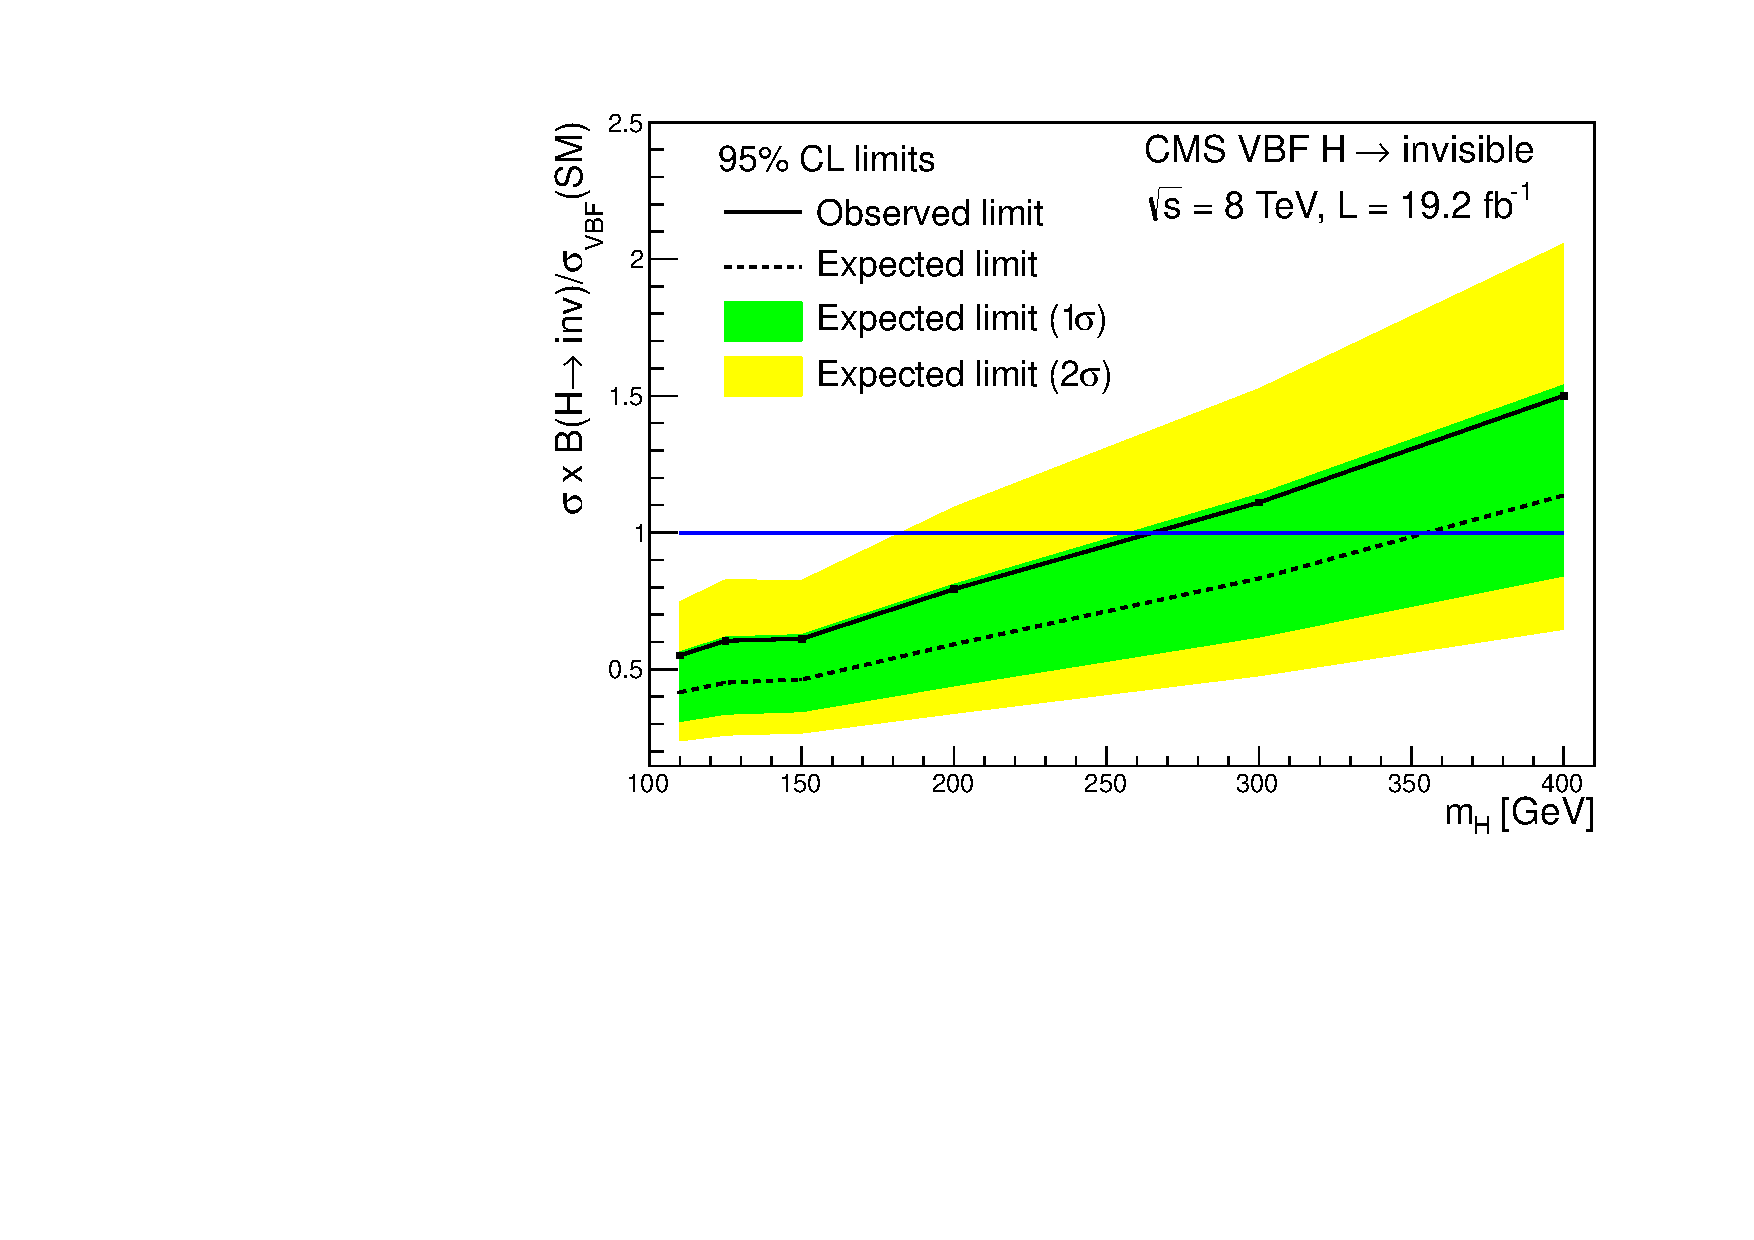
\includegraphics[clip=true,trim=0 0 0 20,width=.5\textwidth]{TalkPics/pubcommpoints260115/vbflimit.pdf}
  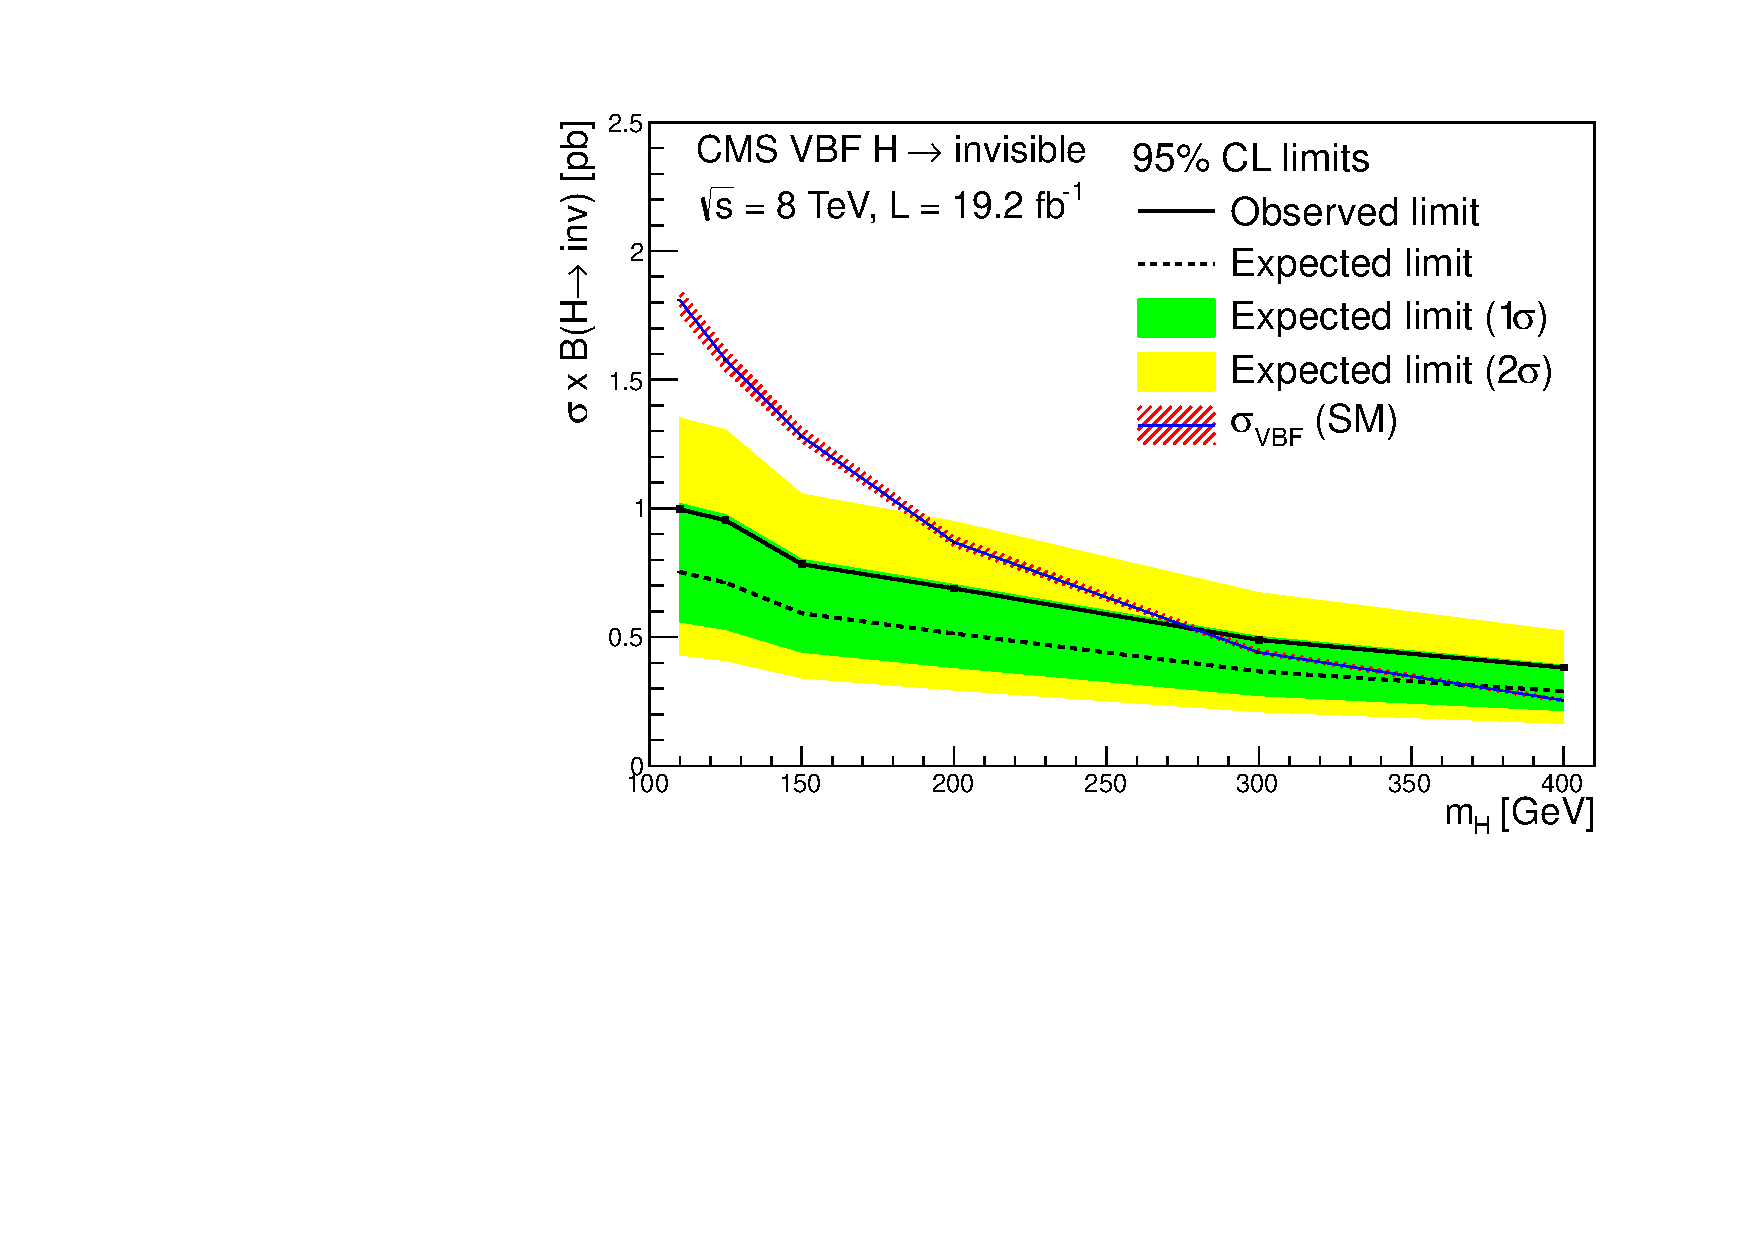
\includegraphics[clip=true,trim=0 0 0 20,width=.5\textwidth]{TalkPics/pubcommpoints260115/vbfxslimit.pdf}
\end{frame}

\begin{frame}
  \frametitle{Combination with ZH}
  \centering
  \begin{block}{}
    \scriptsize
    \begin{itemize}
    \item The improvement to the combined result is greater than that in VBF only
    \item[-] Prompt limit was 0.58 (0.44) observed (expected)
    \item[-] With the parked VBF analysis this becomes 0.48(0.39)
    \item We believe this to be due to the new VBF best fit signal strength being more similar to that from ZH.
    \end{itemize}
  \end{block}
\end{frame}

\begin{frame}
  \frametitle{Combination with ZH}
  \centering
  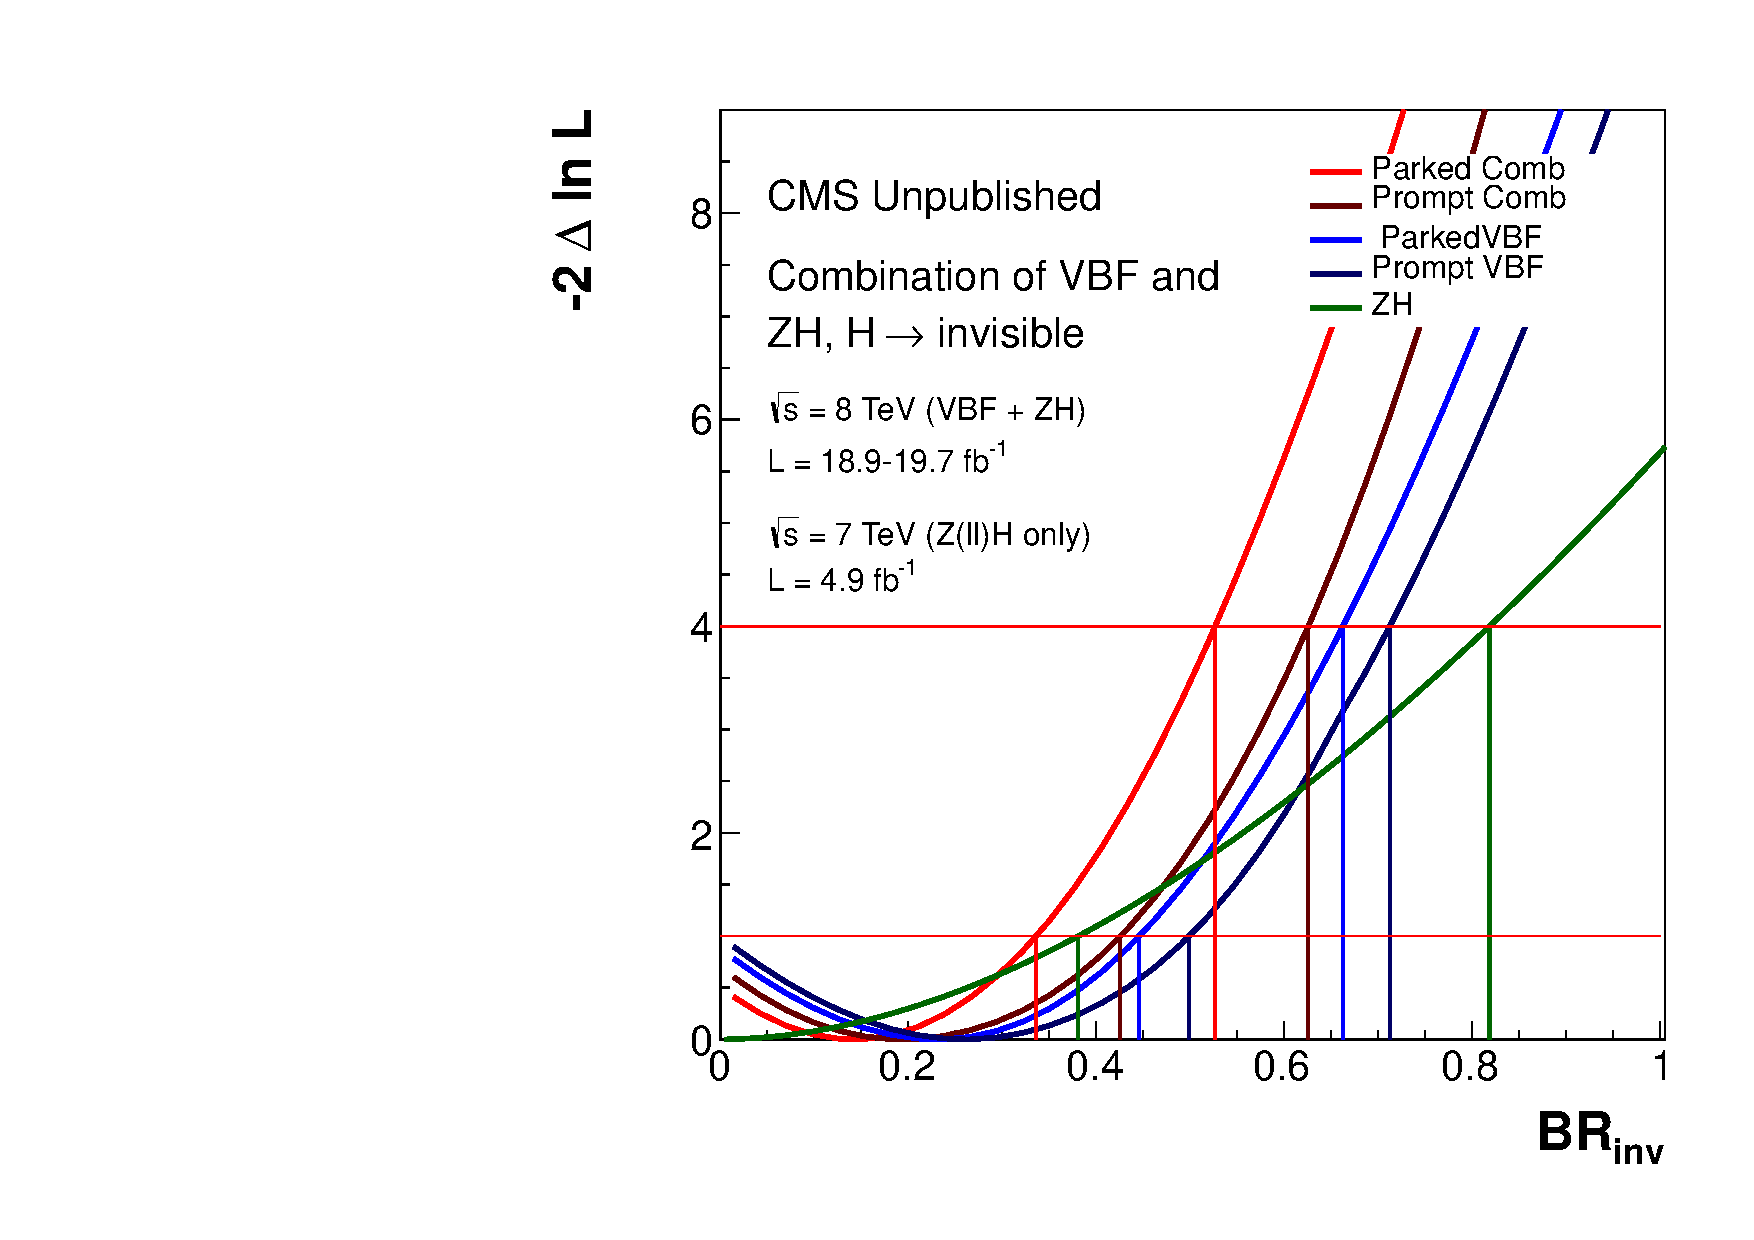
\includegraphics[width=.65\textwidth]{TalkPics/pubcommpoints260115/scan.pdf}  
\end{frame}

\begin{frame}
  \frametitle{Summary}
  \label{lastframe}
  \begin{block}{}
    \scriptsize
    \begin{itemize}
    \item The parked data VBF analysis allows us to set our first direct limit on B(H$\rightarrow$ inv) below 50\%
    \item[-] a relative improvement of 17\% on the previous combined observed limit and 11\% on the expected limit
    \item This is the run I legacy result not an intermediate step
    \item Reduced trigger acceptance means that this is likely to be the strongest limit until at least late 2016
    \item We therefore believe that this analysis warrants a journal article
    \end{itemize}
  \end{block}
\end{frame}

\begin{frame}
  \frametitle{Backup}
\end{frame}

\end{fmffile}
\end{document}
